\chapter{Aspetti di Domain Driven Design}
    \section{Individuazione Domains map e core domain}	
    All'interno del Knowledge Krunching, domande significative sono state fatte per capire i concetti fondamentali del dominio.
    Non tutte le parti hanno egual importanza, in questo capitolo si cerca individuare il core domain. Infatti, è necessario ridurre la complessità focalizzandosi su quelle più importanti, ciò aiuta a diminuire la difficoltà globale.
    Inoltre c'è da specificare che il core domain non va confuso con l’organizzazione dell'azienda, nel nostro caso il software va a risolvere un problema mirato, non coincidente con l'intero ambito aziendale.
    Ulteriore attenzione è stata fatta al fatto che il core possa cambiare con il tempo.
    
    %TABELLA DOMINI
    \begin{figure}[ht]
        \caption{Rappresentazione grafica dei domini}
        \centering
        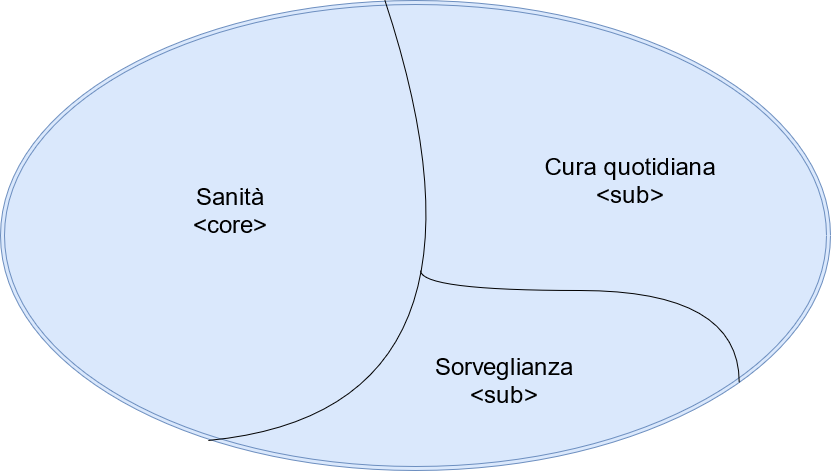
\includegraphics[width=0.5\textwidth]{DrawIo/domainsMap.png}
    \end{figure}
    

    Sono stati identificati tre domain, dove:
    
    \begin{itemize}
        \item \textbf{Sanità} è il \textbf{core domain}. Contiene tutta la logica e le funzioni utili a determinare lo stato di salute dell'animale, partendo dai soli dati vitali.
        
        \item \textbf{Cura quotidiana} è il \textbf{support domain}. Tramite la cura e le informazioni ricavate dalle azioni quotidiane dell'animale supporta il \textbf{core domain} nell'analisi di anomalie quali patologie, problemi di salute o comportamentali.
        
        \item \textbf{Sorveglianza} è il sub domain relativo alla gestione e monitoraggio video del canile.
    \end{itemize}
    \section{Identificazione dei Subdomain}
    \section{Definizione dei Bounded Context}
    \section{Definizione delle Context Map}